% Make nice A4 pages for print:
%\usepackage{pgfpages}
%\pgfpagesuselayout{resize to}[a4paper,border shrink=5mm,landscape]

\beamertemplatenavigationsymbolsempty

\setbeamertemplate{bibliography item}[text]

\usepackage[type={CC},modifier={by-sa},version={4.0}]{doclicense}

\usepackage[utf8]{inputenc}
\usepackage{hyperref}
\usepackage{breakurl}
\usepackage{graphicx}
\usepackage{pgfplots}
\usepackage{pgf}
\usepackage{tikz}
\usetikzlibrary{positioning}
\usetikzlibrary{arrows}
\usetikzlibrary{decorations.markings}
\usetikzlibrary{calc}
\usetikzlibrary{matrix}
\usetikzlibrary{shapes}
\usetikzlibrary{decorations.pathmorphing}
\usetikzlibrary{fit}
\usetikzlibrary{backgrounds}
\usetikzlibrary{plotmarks}
\usepackage{stmaryrd}
\usepackage{listings}
\usepackage{pdflscape}
\usepackage{perpage}
\usepackage{appendixnumberbeamer}

%\usepackage[thmmarks,amsmath,amsthm]{ntheorem} % already included in beamer
\usepackage{thm-restate}

\usepackage[sort&compress,numbers]{natbib}  % to be have \citet, \citeauthor, \citeyear

\MakePerPage{footnote}

\tikzstyle{o}=[r,ppBlue]
\tikzstyle{r}=[thick,rectangle,align=center]
\tikzstyle{t}=[r,ppTrans] %,font=\bfseries]
\tikzstyle{dd}=[densely dashed]
\tikzstyle{n}=[r,ppBlue]
\tikzstyle{p}=[r,ppRed]
\tikzstyle{ppRed}  =[draw=red,  fill=  red!20]
\tikzstyle{ppBlue} =[draw=blue, fill= blue!20]
\tikzstyle{ppGreen}=[draw=green,fill=green!20]
\tikzstyle{ppTrans}=[draw=none, fill=none]

\usetheme{Warsaw}

\useoutertheme[subsection=true]{smoothbars}
%\useoutertheme[subsection=false]{miniframes}

\definecolor{bblue}{HTML}{D7DF01}	% yellow-ish actually, for better black/white printing
\definecolor{rred}{HTML}{C0504D}
\definecolor{ggreen}{HTML}{9BBB59}
\definecolor{ppurple}{HTML}{9F4C7C}
\definecolor{lightgray}{rgb}{0.3,0.3,0.3}
\definecolor{lightergray}{rgb}{0.9,0.9,0.9}
\definecolor{UniBlue}{RGB}{83,121,170}

\DeclareTextFontCommand\textintro{\normalfont\bfseries\itshape} % nice!
\newcommand{\intro}[2][]
{%
	\textintro{#2}%
}
\newcommand{\empha}[2][]
{%
	\emph{#2}%
}

%\theoremstyle{plain}
\newcounter{reqcounter}
\newtheorem{requirement}[reqcounter]{Requirement}

%setbeamercolor{structure}{fg=violet}

\makeatletter
\def\th@task{%
    \normalfont % body font
    \setbeamercolor{block title example}{bg=orange,fg=white}
    \setbeamercolor{block body example}{bg=orange!20,fg=black}
    \def\inserttheoremblockenv{exampleblock}
  }
\makeatother

\theoremstyle{task}
\newtheorem{task}{Task}

\newenvironment{assignment}%
{%\setbeamercolor{background canvas}{bg=violet}%
%\setbeamercolor{structure}{fg=cyan!90!black}%
 \setbeamercolor{frametitle}{bg=orange,fg=white}
\begin{frame}}%
{\end{frame}}%

\AtBeginSection[]{
  \begin{frame}
  \vfill
  \centering
  \begin{beamercolorbox}[sep=8pt,center,shadow=true,rounded=true]{title}
    \usebeamerfont{title}\insertsectionhead\par%
  \end{beamercolorbox}
  \tableofcontents
  \vfill
  \end{frame}
}




\pgfplotsset{compat=1.14}
\author{Markus Raab}


\title{L03 Configuration Integration}
\date{24.03.2021}

\begin{document}

%%%%%%%%%%%%%%%%%%%%%%%%%%%%%%%%%%%%%%%%%% 
\section{Configuration Libraries}

\begin{frame}
	\frametitle{Configuration Access APIs}

	\Large
	\ExecuteMetaData[../book/background.tex]{definition-api}

	\ExecuteMetaData[../book/background.tex]{definition-configuration-access}
\end{frame}

\begin{frame}[fragile]
	\frametitle{Configuration Access APIs}

	\begin{itemize}[<+-| alert@+>]
	\item ^char * getenv (const char * key)^
	\item ^ConfigStatus xf86HandleConfigFile(Bool autoconf)^
	\item ^long pathconf (const char *path, int^ ^name)^
	\item ^long sysconf (int name)^
	\item ^size_t confstr (int name, char *buf, size_t len)^
	\end{itemize}
\end{frame}

\begin{frame}[fragile]
	\frametitle{Configuration Access Points}
	\ExecuteMetaData[../book/background.tex]{definition-configuration-access-points}

	\begin{code}[language=Cpp,gobble=4,showspaces=no]
	int main()
	{
		getenv ("PATH");
	}
	\end{code}
\end{frame}

\begin{frame}[fragile]
	\frametitle{Configuration Libraries}
	\ExecuteMetaData[../book/background.tex]{definition-configuration-library}

	Trends:
	\begin{itemize}[<+-| alert@+>]
	\item flexibility to configure configuration access (e.g., \url{https://commons.apache.org/proper/commons-configuration/})
	\item more type safety (e.g., \url{http://owner.aeonbits.org/}, code generation)
	\item specifications and introspection (gsettings, XML/JSON, Elektra)
	\item configuration integration (UCI, Augeas, Elektra)
	\end{itemize}
\end{frame}

\begin{frame}
	\frametitle{Current Situation}
	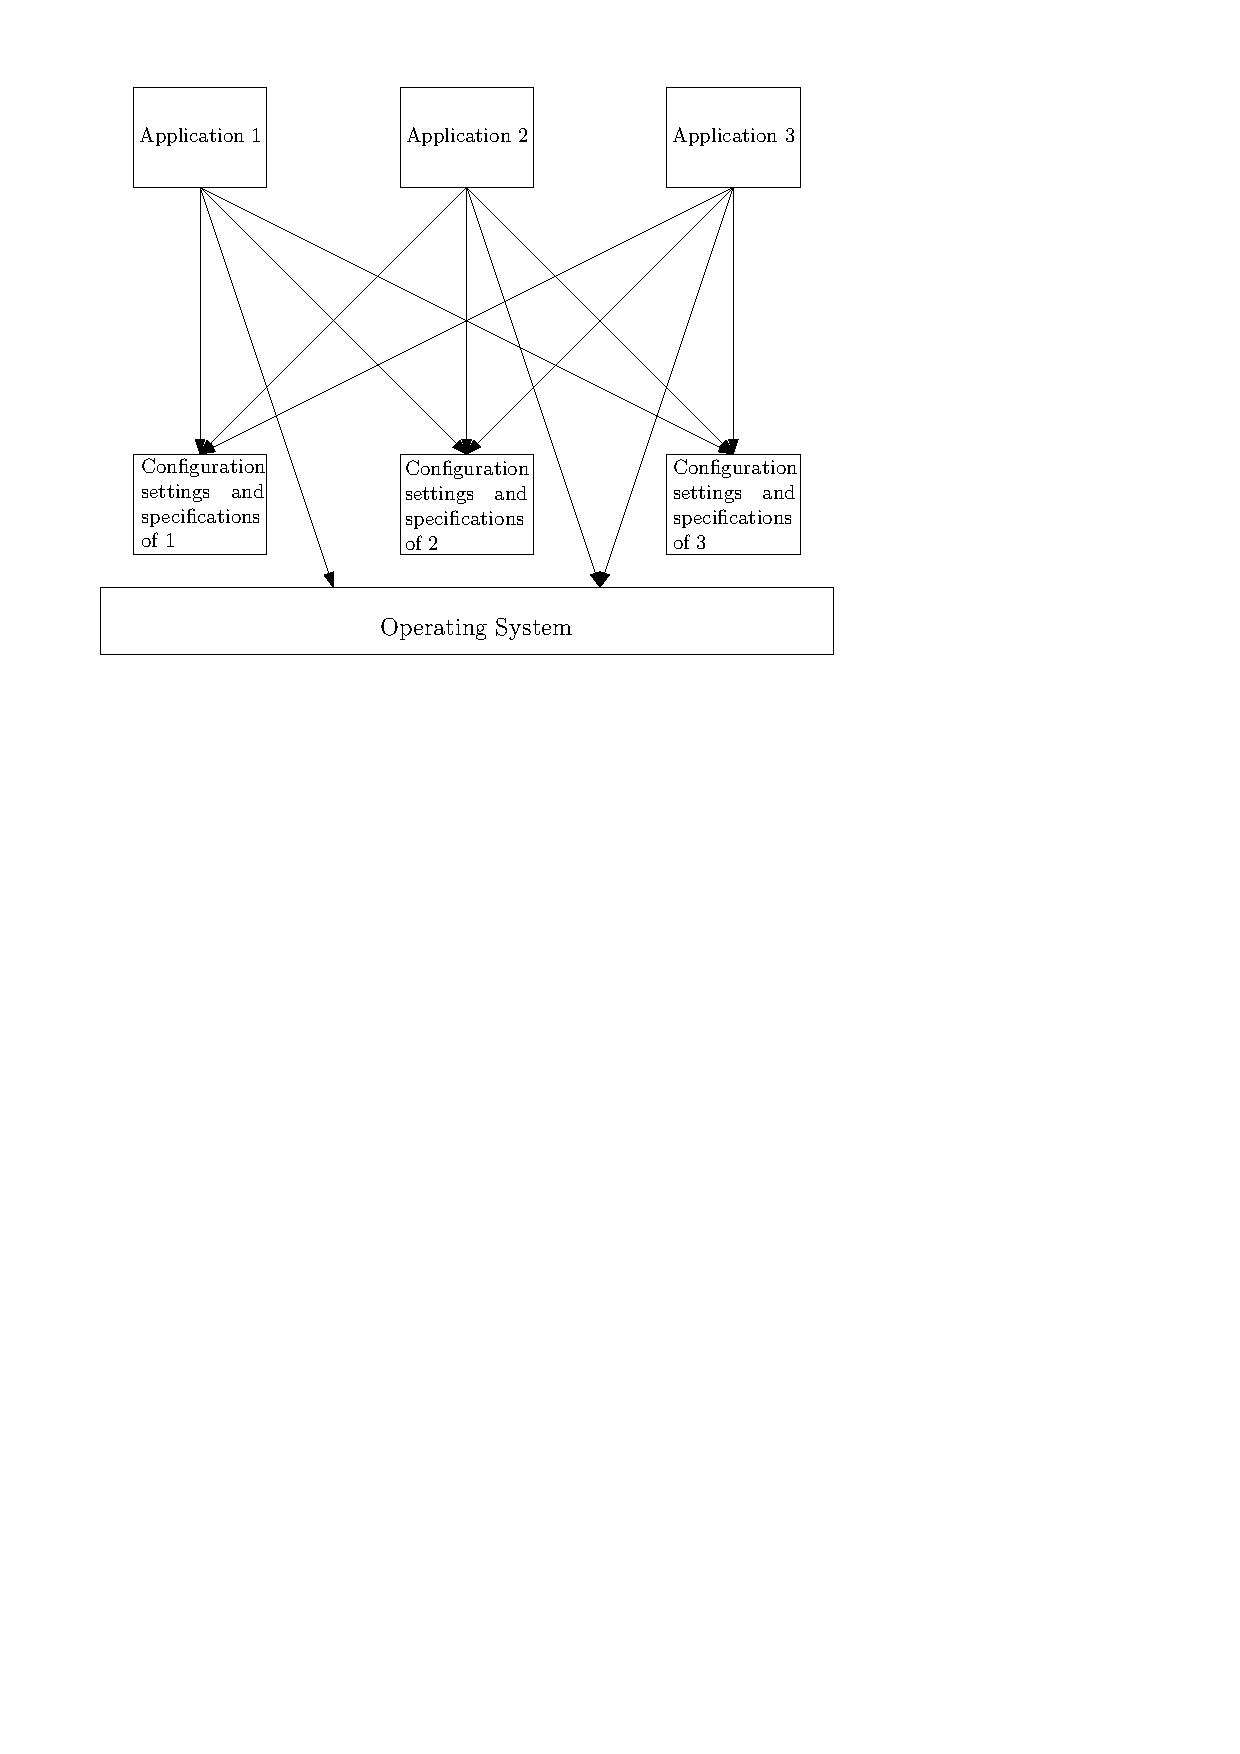
\includegraphics[scale=0.7]{cursituation}
\end{frame}

\begin{frame}
	\frametitle{Wanted Situation}
	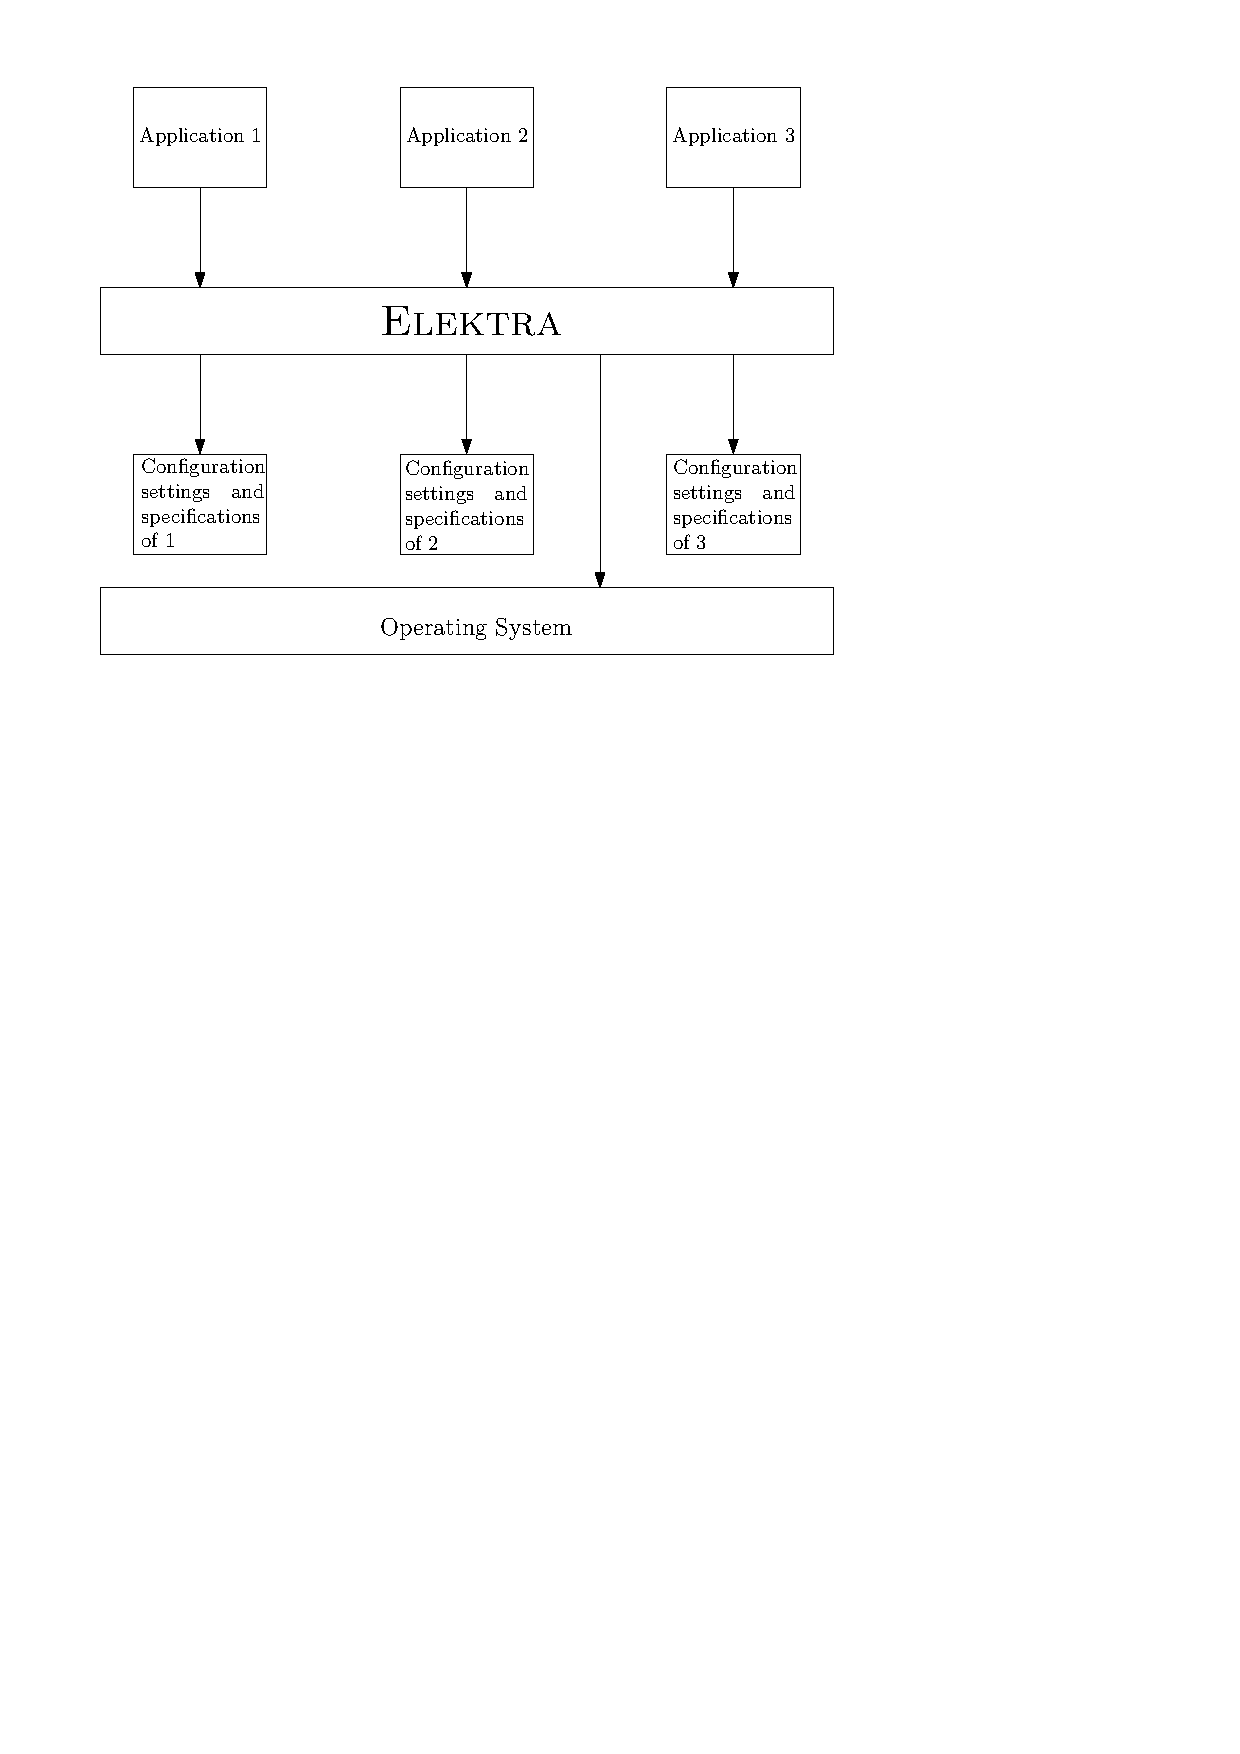
\includegraphics[scale=0.7]{wantsituation}
\end{frame}


%%%%%%%%%%%%%%%%%%%%%%%%%%%%%%%%%%%%%%%%%% 
\section{Lightweight to Strong Integration}

\begin{frame}[fragile]
	\frametitle{Lightweight Integration}

	Specify already-existing configuration files:
	\begin{code}[language=Cpp,gobble=4,showspaces=no]
	[ntp]
	  mountpoint:=ntp.conf
	  infos/plugins:=ntp
	\end{code}

	\vspace{1cm}
	Works well for configuration management tools.
\end{frame}

\begin{frame}[fragile]
	\frametitle{Medium Integration}

	Having frontends that implement existing \textbf{APIs} decouple applications from each other.
	These applications continue to use their specific configuration accesses, but \elektra{} redirects their configuration accesses to the shared key database.

	Possible APIs:
	\begin{itemize}[<+-| alert@+>]
	\item ^getenv^
	\item open/close of configuration files
	\end{itemize}

	\pause[\thebeamerpauses]
	\vspace{1cm}

	Also needs application-specific specifications.
\end{frame}

\begin{frame}[fragile]
	\frametitle{Strong Integration}

	Change the application so that it directly uses Elektra.

	Advantages:
	\begin{itemize}[<+-| alert@+>]
	\item Elektra's features always available
	\item more type safety
	\item administrators can choose configuration file formats
	\item notification and logging
	\item only one parser involved
	\item no specification for binding needed
	\item no built-in defaults: everything is introspectable
	\end{itemize}
\end{frame}

\begin{frame}[fragile]
	\frametitle{Strong Integration}

	Different implementations strategies:

	\begin{itemize}[<+-| alert@+>]
	\item have some application-specific API which uses ^KeySet^
	\item use one of KeySet's language bindings
	\item use Elektra's high-level API (currently only C)
	\item use code generation
	\end{itemize}
\end{frame}

\begin{frame}[fragile]
	\frametitle{Strong Integration}
	Examples:
	\begin{itemize}
	\item LCDproc
	\item Oyranos
	\item for GNOME: ^gsettings^
	\item for KDE: ^kconfig^
	\end{itemize}
\end{frame}



\section{Sharing Configuration}

\begin{frame}
	\begin{itemize}
	\item idea: make default values better
	\item generalization of sharing configuration values
	\item examples: language settings, default printer, \dots
	\end{itemize}
	\pause
	\vspace{1cm}
	Can be derived from:
	\begin{itemize}
	\item other configuration settings (override/fallback)
	\item context~\cite{raab2017introducing}
	\item hardware/system (problem with dependences)
	\pause
	\vspace{1cm}
	\item XServer vs.\ gpsd
	\end{itemize}
\end{frame}

\begin{frame}[fragile]
	\frametitle{Examples}
	Context:
	\begin{code}[gobble=4]
	[slapd/threads/listener]
	context:=/slapd/threads/%cpu%/listener
	\end{code}

	\pause
	\vspace{1cm}
	Calculation with conditionals plugin
	\\ (e.g., switch off GPS if battery low):
	\begin{code}[gobble=4]
	[gps/status]
	assign:=(battery > 'low') ? ('on') : ('off')
	\end{code}
\end{frame}

\section{Meeting}

\begin{frame}
	\begin{alertblock}{Question}
	How do we get such an specification now?
	\end{alertblock}

	\pause
	\begin{exampleblock}{Answer}
	Elektrify: Make the application use a configuration library that has support for configuration specifications.
	\end{exampleblock}
\end{frame}

\begin{frame}
	\begin{task}
	Which configuration access APIs do you know? \\
	What are the differences between these APIs?
	\end{task}
\end{frame}

\appendix

\begin{frame}[allowframebreaks]
	\bibliographystyle{plainnat}
	\bibliography{../shared/elektra.bib}
\end{frame}


\end{document}
